%%%%%%%%%%%%%%%%%%%%%%%%%%%%%%%%%%%%%%%%%%%%%%%%%%%%%%%%%%%%%%%%%%
%%
%%                Proceedings of the annual meeting 
%%               of the French Astronomical Society  
%%      Société Française d'Astronomie et d'Astrophysique  (SF2A)
%% 
%%%%%%%%%%%%%%%%%%%%%%%%%%%%%%%%%%%%%%%%%%%%%%%%%%%%%%%%%%%%%%%%%%
%%
%% These proceedings are published electronically in English.
%%
%% The proceedings must be prepared using the present template.
%% Please follow rigorously the instructions. 
%%
%% The recommended number of pages is:
%%   * Review -> 6 pages or more
%%   * Oral contribution ->  4 pages or more
%%   * Poster -> 2 pages or more
%% 
%% All your files must named as follows:
%%     surname.tex, surname.bib, surname_fig1.pdf, surname_fig2.pdf...
%%
%% And if you have several contributions:
%%     surname1.tex, surname2.tex ... etc
%%     surname1_fig1.pdf, surname2_fig1.pdf, ... etc
%%
%% Please provide only PDF figures 
%% To convert figures from eps to pdf, you may use epstopdf
%%
%% Once completed, please send your proceedings as a single tar.gz (surname.tar.gz) 
%% file at secretariat@sf2a.eu before Friday 30th September 2016 
%% (Please mention the subject: "Proceedings SF2A 2016").  
%% 
%% Thank you !
%%
%%%%%%%%%%%%%%%%%%%%%%%%%%%%%%%%%%%%%%%%%%%%%%%%%%%%%%%%%%%%%%%%%%
\documentclass{sf2a-conf2016}
\usepackage{graphicx}
\usepackage{hyperref}
\usepackage[]{natbib}  
\usepackage{epstopdf}
\renewcommand{\thefootnote}{\fnsymbol{footnote}}
\def\BibTeX{{\rm B\kern-.05em{\sc i\kern-.025em b}\kern-.08em
    T\kern-.1667em\lower.7ex\hbox{E}\kern-.125emX}}
\bibpunct{(}{)}{;}{a}{}{,}  %%%%%%%%%%%%%  A&A bibliography style
%%-----------------------------------------------------------------
%%         your macros below:
%%
\newcommand{\kms}{{\mathrm{km~s^{-1}}}}
\newcommand{\kpc}{{\mathrm{kpc}}}
%%-----------------------------------------------------------------
%% ajouter Guilaine Lagache, Anaelle Maury,
%% Helene Roussel, Jean-Francois Lestrade, Juan Soler and Hervé Aussel.
%%%%%%%%%%%%%%%--BODY--%%%%%%%%%%%%%%%%%%

\begin{document}

\TitreGlobal{SF2A 2016}

%%-----------------------------------------------------------------
%%      the top matter
%%

\title{NIKA2, a dual-band millimetre camera on the IRAM 30~m telescope to map the cold universe }

\runningtitle{NIKA2 status}


%\author{A. Author1}\address{Timberland Observatory, 34560 City, Neverland}

%\author{J.-P. Author2}\address{Institute XYZ, 1299 City, OtherLand}


\author{F.-X.~D\'esert} \address{Institut de Plan\'etologie et d'Astrophysique
  de Grenoble, Univ. Grenoble Alpes, CNRS, IPAG, F-38000 France}
%IPAG 1

\author{R.~Adam$^{2,} $} \address{Laboratoire de Physique Subatomique et de
  Cosmologie, Universit\'e Grenoble Alpes, CNRS/IN2P3, 53, avenue des Martyrs,
  Grenoble, France} \address{Laboratoire Lagrange, Universit\'e C\^ote d'Azur,
  Observatoire de la C\^ote d'Azur, CNRS, Blvd de l'Observatoire, CS 34229,
  06304 Nice cedex 4, France}
%LPSC 2,OCA 3

\author{P.~Ade} \address{Astronomy Instrumentation Group, University of Cardiff,
  UK} %Cardiff 4

\author{ P.~Andr\'e} \address{Laboratoire AIM, CEA/IRFU, CNRS/INSU,
    Universit\'e Paris Diderot, CEA-Saclay, 91191 Gif-Sur-Yvette,
    France} % CEA 5

\author{ H.~Aussel$^{5} $}

\author{  A.~Beelen} \address{Institut d'Astrophysique Spatiale (IAS), CNRS
  and Universit\'e Paris Sud, Orsay, France} % IAS 6

\author{  A.~Beno\^it} \address{Institut N\'eel, CNRS and Universit\'e
  Grenoble Alpes, France} % Neel 7

\author{  A.~Bideaud$^{7}$}

\author{ N.~Billot} \address{Institut de RadioAstronomie Millim\'etrique
  (IRAM), Granada, Spain} % IRAME 8

\author{  O.~Bourrion$^{2}$}

\author{  M.~Calvo$^{7}$} 

\author{  A.~Catalano$^{2}$}

\author{  G.~Coiffard} \address{Institut de RadioAstronomie Millim\'etrique
  (IRAM), Grenoble, France} % IRAMF 9

\author{  B.~Comis$^{2}$} 

\author{  S.~Doyle$^{4}$}

\author{  J.~Goupy$^{7}$}

\author{  C.~Kramer$^{8}$}

\author{ G.~Lagache} \address{Aix Marseille Universit\'e, CNRS, LAM
  (Laboratoire d'Astrophysique de Marseille) UMR 7326, 13388, Marseille,
  France}

\author{  S.~Leclercq$^{9}$}

\author{ J.-F.~Lestrade} \address{LERMA, CNRS, Observatoire de Paris, 61 Avenue de l'Observatoire, Paris, France}

\author{  J.F.~Mac\'ias-P\'erez$^{2}$}

\author{ A.~Maury$^{5}$}

\author{  P.~Mauskopf$^{4,} $} \address{School of Earth and Space Exploration
  and Department of Physics, Arizona State University, Tempe, AZ 85287}

\author{  F.~Mayet$^{2}$}

\author{  A.~Monfardini$^{7}$}

\author{  F.~Pajot$^{6}$}

\author{  E.~Pascale$^{4}$} 

\author{  L.~Perotto$^{2}$}

\author{  G.~Pisano$^{4}$} 

\author{  N.~Ponthieu$^{1}$}

\author{  V.~Rev\'eret$^{5}$}

\author{  A.~Ritacco$^{2}$}

\author{  L.~Rodriguez$^{5}$}

\author{  C.~Romero$^{9}$}

\author{ H.~Roussel} \address{Institut d'Astrophysique de Paris, CNRS
  (UMR7095), Sorbonne Universit\'es, UPMC Univ. Paris 06, 98 bis Boulevard
  Arago, F-75014, Paris, France}

\author{  F.~Ruppin$^{2}$}

\author{ J.~Soler$^{5}$}

\author{  K.~Schuster$^{9}$}

\author{  A.~Sievers$^{8}$}

\author{  S.~Triqueneaux$^{7}$}

\author{  C.~Tucker$^{4}$}

\author{  R.~Zylka$^{9}$}

%% IF Author3 has the same affiliation than Author1:
%\author{C.\,E. Author3$^1$}

%% IF Author3 has its own affiliation:
%\author{C.\,E. Author3}\address{Dept. of Chess, University of Games, 35101 Las Vegas, Monaco} 

%% IF Author3 has two affiliations, the one of Author1 and a second one:
%\author{C.\,E. Author3$^{1,}$}\address{Dept. of Chess, University of Games, 35101 Las Vegas, Monaco} 


%% Keep this line, even if the page will be settled afterwards.
\setcounter{page}{237}



%%-----------------------------------------------------------------

\maketitle

%%-----------------------------------------------------------------
%%        The abstract
%% 
%%  Warning!  within the abstract:
%%  - do not use macros. 
%%  - do not use commands like: \cite, \citet, \citep ... etc.

\begin{abstract}
  A consortium led by Institut N\'eel (Grenoble) has just finished installing
  a new powerful millimetre camera NIKA2 on the IRAM 30~m telescope. It has an
  instantaneous field-of-view of 6.5~arcminutes at both 1.2 and 2.0 mm with
  polarimetric capabilities at 1.2~mm. NIKA2 provides a near diffraction-limited
  angular resolution (resp. 12 and 18 arcseconds). The 3 detector arrays are
  made of more than 1000 KIDs each. KIDs are new superconducting devices
  emerging as an alternative to bolometers. The commissionning is ongoing in
  2016 with a likely opening to the IRAM community in early 2017. NIKA2 is a
  very promising multi-purpose instrument which will enable many
  scientific discoveries in the coming decade.
\end{abstract}


%% Insert the keywords (to appear in the ADS indexing)
%% Keywords must be separated by a comma
\begin{keywords}
Camera, millimetre astronomy, cosmology, galaxies, star formation,
interstellar dust
\end{keywords}

%%-----------------------------------------------------------------


\section{Introduction}
%%---------------------
The golden age of (sub)millimetre astronomy started with the two flagship
space missions Herschel and Planck. It is now ongoing with the two world-class
(sub)millimetre interferometers ALMA and NOEMA. Whereas Herschel and Planck
provided surveys of a large portion or all of the sky at medium angular
resolution (35~arcsec. at 500~micron for Herschel and 5~arcmin at 1~mm for
Planck), the ground-based interferometers can dig deeply at high angular
resolution (sub-arcsecond), but only on very tiny spots (around 20~arcseconds
at 1~mm) of the sky. The IRAM 30~m radiotelescope, a leading millimetre
facility in Spain, near Granada, can fill the angular scale gap. For that
purpose, a wide-field camera is necessary. A consortium of laboratories in
France and UK, along with IRAM, has just built and installed such a camera
called NIKA2~\citep[more details given
in][\href{http://ipag.osug.fr/nika2}{see also
  http://ipag.osug.fr/nika2}]{2016arXiv160508628C}.
  
\section{A description of NIKA2}
%%-------------------------
The camera is based on novel detectors. Kinetic Inductance Detectors (KIDs)
are supraconducting devices~\citep{2003Natur.425..817D,2006SPIE.6275E..1OD} that
see their electrical properties change with incoming light. The kinetic
inductance is modified when Cooper pairs are broken by photons of sufficient
energy. KIDs are proving to be an alternative to bolometers with specific
advantages: time constant (less than a millisecond), low sensitivity to the
cooler temperature (a thousand times less than for a bolometer), and ease to
manufacture (a single aluminum layer on a silicon wafer). Each detector is
wired to be a high-efficiency RLC resonator coupled by a linefeed to the
readout. The signal can thus be frequency-multiplexed by a factor of at least
150, each KID having its own resonant frequency. Moreover the detector
resonance frequency is linearly dependent on the incoming photon flux. A
complex readout system is required to simultaneously measure all the detectors
at a sampling rate of up to 100~Hz~\citep{bourrion2011}. Since 2009, these
properties have been checked on the sky with the NIKA prototype
camera~\citep{monfardini2010,monfardini2011,Calvo2013,catalano2014} at the
IRAM 30~m telescope. Figure~\ref{fig1-2} (left panel) shows one of the two
NIKA2 1~mm arrays. The sampling of the sky by each planar array is of
$F.\lambda\simeq 0.7-1$.

%% two figures side by side
%%
\begin{figure}[ht!]
 \centering
 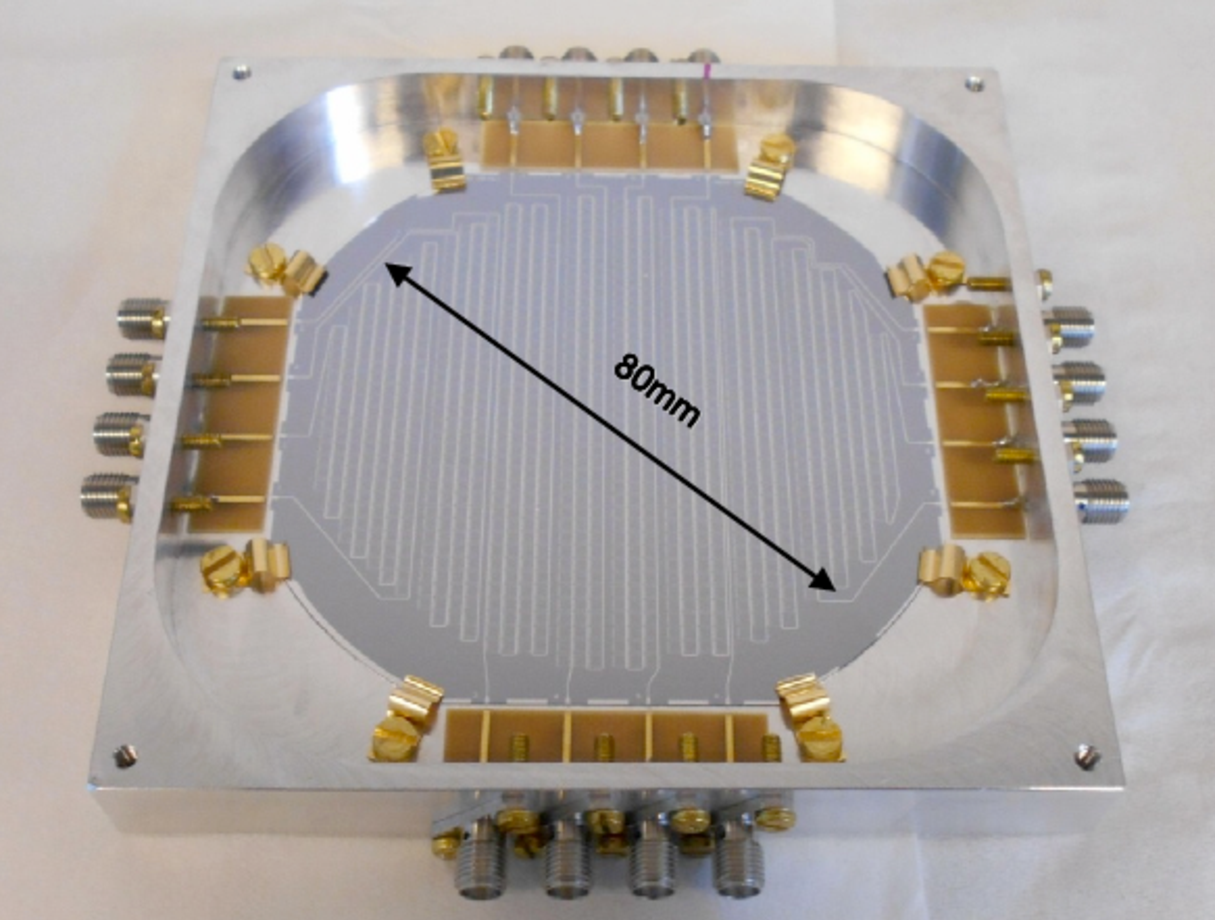
\includegraphics[width=0.48\textwidth,clip]{desert_fig1}%      
 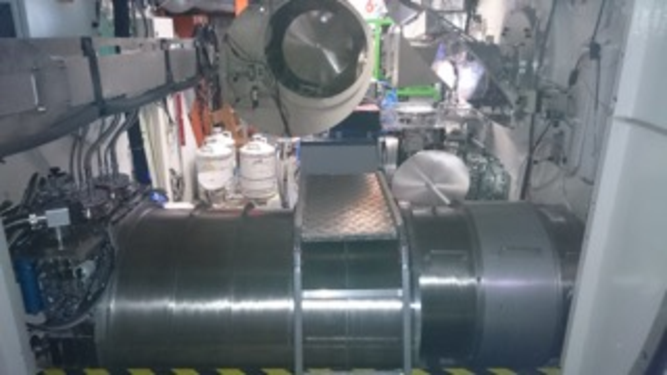
\includegraphics[width=0.48\textwidth,clip]{desert_fig2}      
 \caption{{\bf Left:}~NIKA2 1~mm array containing more than 1000 KIDs. It is
   made of a single layer of aluminum on a silicon wafer. Aluminum is a
   supraconductor below 1~K. Feedlines are seen meandering around the
   detectors. The readout connectors can be seen on the sides: a pair of
   connectors correspond to the input and output of one feedline and there are
   8 readouts needed to read that array. {\bf Right:}~The NIKA2 cryostat in
   the Nasmyth cabin of the IRAM 30~m radiotelescope. }
  \label{fig1-2}
\end{figure}


Most of NIKA2 is made of two 4~K pulse-tube cryocoolers and a closed-cycle
$^3$He-$^4$He dilution fridge so that these detectors can function at
typically 150~mK. The NIKA2 cryostat provides a continuous cooling (no duty
cycles) for the whole duration of each observing campaign (up to several
months). The optics is made of polyethylene lenses with a near-telecentric
system that focuses light on the plane detectors. Filtering (high-frequency
cut-off, bandpass) is done via mesh filters~\citep{2006SPIE.6275E..0UA}. A
dichroic splits the 1 and 2~mm light. Then, a polarizing capability is
obtained by having a cold polarizing grid at 45~deg. from the incoming 1~mm
light splitting the two linear polarizations onto the two 1~mm arrays. When
one wishes NIKA2 to be in the polarization observing mode, a removable
half-wave plate can be slid in front of the cryostat. This system was used
with NIKA~\citep{2016arXiv160902042R} and provides a continuous rotation of
the polarization axis so that Stokes parameters for the linear polarization
can be retrieved. Figure~\ref{fig1-2} (right panel) shows how the heavy
cryostat (more than 1.3~tons) fits into the Nasmyth cabin of the IRAM 30~m
radiotelescope. A new optical system (M3 and M4 mirrors) had to be designed to
accommodate the NIKA2 field-of-view.


\section{The performance of NIKA2}


NIKA2 provides an instantaneous circular field of view with a
6.5~arcmin. diameter on the sky in a simultaneous way in the two broad
atmospheric bands at 260~GHz (1.2~mm) and 150~GHz (2.0~mm). The angular
resolution is better than 12 and 18~arcsec at resp. 1.2 and 2~mm. The goal
sensitivities are resp. 15 and 10~mJy rms for a point-source in one second of
integration on average across the whole focal plane. The total number of
detectors is about 1100 per array and there are three arrays (two at 1.2~mm
and one at 2~mm). The percentage of valid detectors is above 80~\% (some
detectors cannot be used as their resonant frequencies happen to be too close to
each other). The on-going commissioning is assessing these values with
thorough calibration campaigns and there are no signs that they cannot be
reached.

Maps of the sky can be obtained with a size of up to several degrees by raster
scans: the whole telescope is moving with respect to the map center in a
zig-zag pattern. The secondary mirror is not wobbling. To illustrate NIKA2
early capabilities, we show the maps obtained at 1 and 2~mm in
Fig.~\ref{fig3-4} around the ultracompact HII region NGC~7538, a secondary
calibrator.

%\subsection{ Literature citations}
%%---------------------------------
 
% The following examples illustrate the required style in the main text:
%  \cite{Einstein26} showed that $v_h = 1926 \, \kms$ was not a prime number, as
%  also found previously \citep{Laurel24}. On the other hand, 
%   \citet{1945RvMP...17..120E} followed 
% \citet{Kafka24} and found a better approximation to the
% distance, yielding $d_o = 22 \, \kpc$ \citep[see also][and references therein]{Bohr26,Curie91,deGaulle96}. 
% For frequently cited papers an abbreviated form of citation is
%  recommended, e.g. Paper~I, Paper~II.

% The format for references is the one adopted by A\&A. To set the reference list in the proper format, we encourage you to use \BibTeX~ and the natbib package instead of the standard \verb=\thebibliography= environment.

%\subsection{Footnotes}
%%---------------------

% These should be kept to a minimum and used as 
% usual\footnote{Just like this one.}.


% \subsection{Hyperlinks}

% Hyperlinks can be introduced as follows: \url{http://www.sf2a.eu/}.

% \subsection{Figures}
% %%-------------------

% Please use files in the PDF format, as shown in Fig.~\ref{author1:fig1}. Figures in eps format can be converted to pdf with the command epstopdf (used as ``epstopdf file.eps''). Two figures can be joined together as shown in Fig.~\ref{author1:fig2}. In this case, as illustrated in Fig.~\ref{author1:fig2}, 
% the caption must follow this format (e.g. boldface fonts for the Left and Right items): \textbf{Left:} text
% of the caption for the left panel. \textbf{Right:} text of the caption for the figure on the right hand side. 

% %%
% %% Example of single figure
% %%
% \begin{figure}[ht!]
%  \centering
%  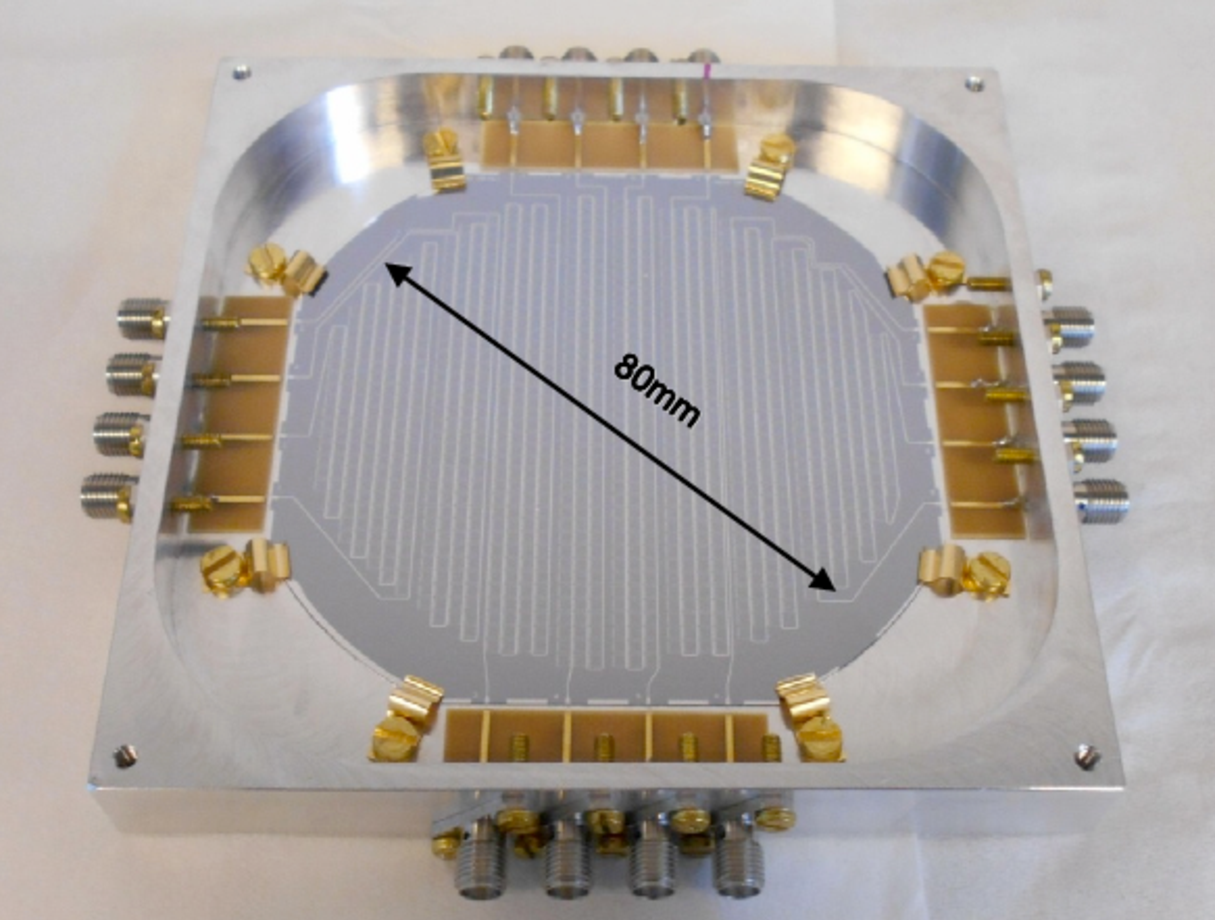
\includegraphics[width=0.8\textwidth,clip]{desert_fig1}      
% %% Note the ABSENCE of the extension .pdf  !
%   \caption{Caption here}
%   \label{author1:fig1}
% \end{figure}

%%
%% Example of two figures side by side
%%
\begin{figure}[ht!]
 \centering
 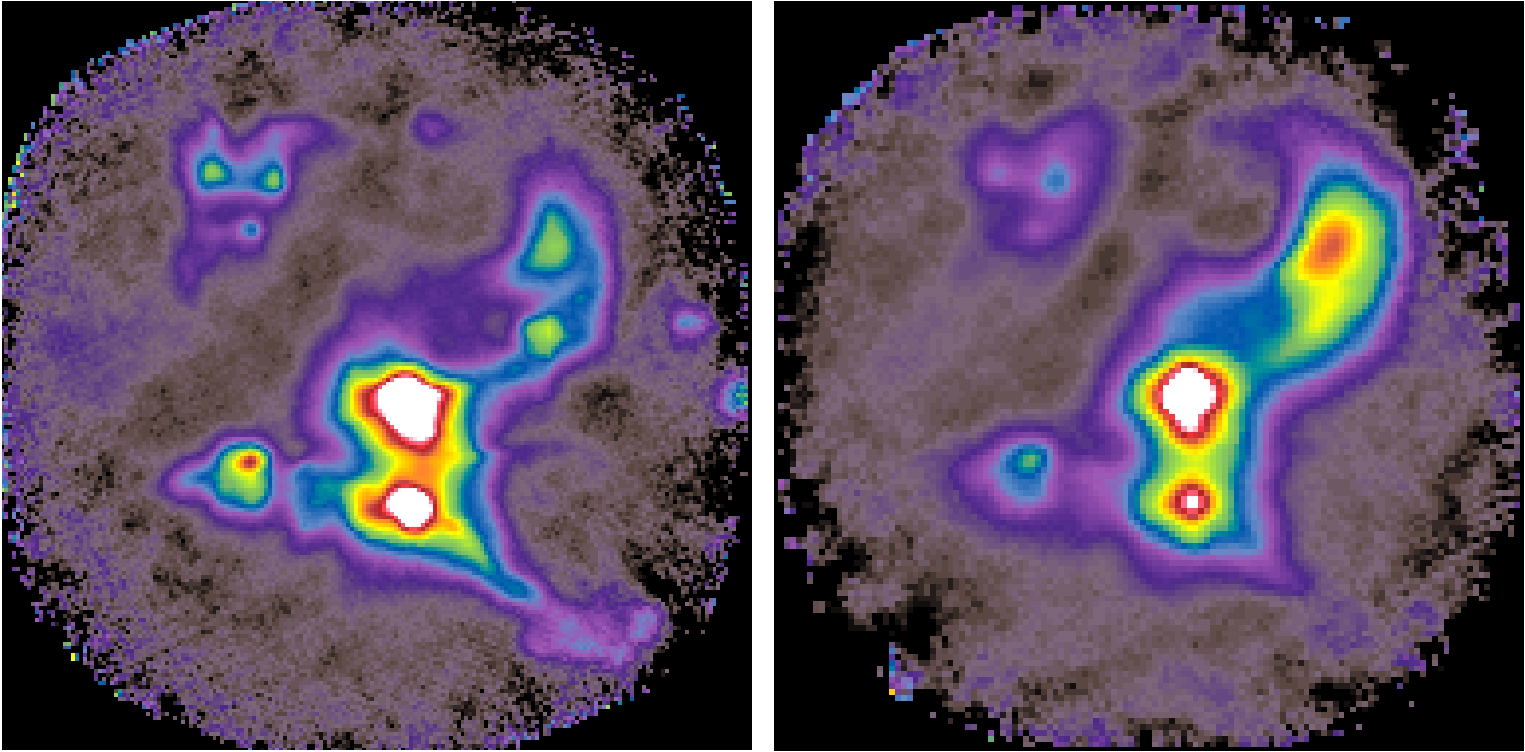
\includegraphics[width=0.8\textwidth,clip]{desert_fig34}%      
 \caption{ RA-Dec maps centered on the ultracompact HII regions NGC~7538 at
   {\bf Left:}~1.2~mm and {\bf Right:}~2~mm. The maps were obtained by using
   the standard NIKA2 IDL-based pipeline and an adaptation of the Scanamorphos
   map-making algorithm~\citep{2013PASP..125.1126R} to NIKA2. The integration
   time was 12 minutes.  The size of the mapped square is 10~arcmin. The
   brightness scale is linear and the maximum is at several Jy per beam. The
   central calibrator is clearly surrounded by many other bright regions.}
  \label{fig3-4}
\end{figure}


% %% Example of two figures side by side
% %%
% \begin{figure}[ht!]
%  \centering
%  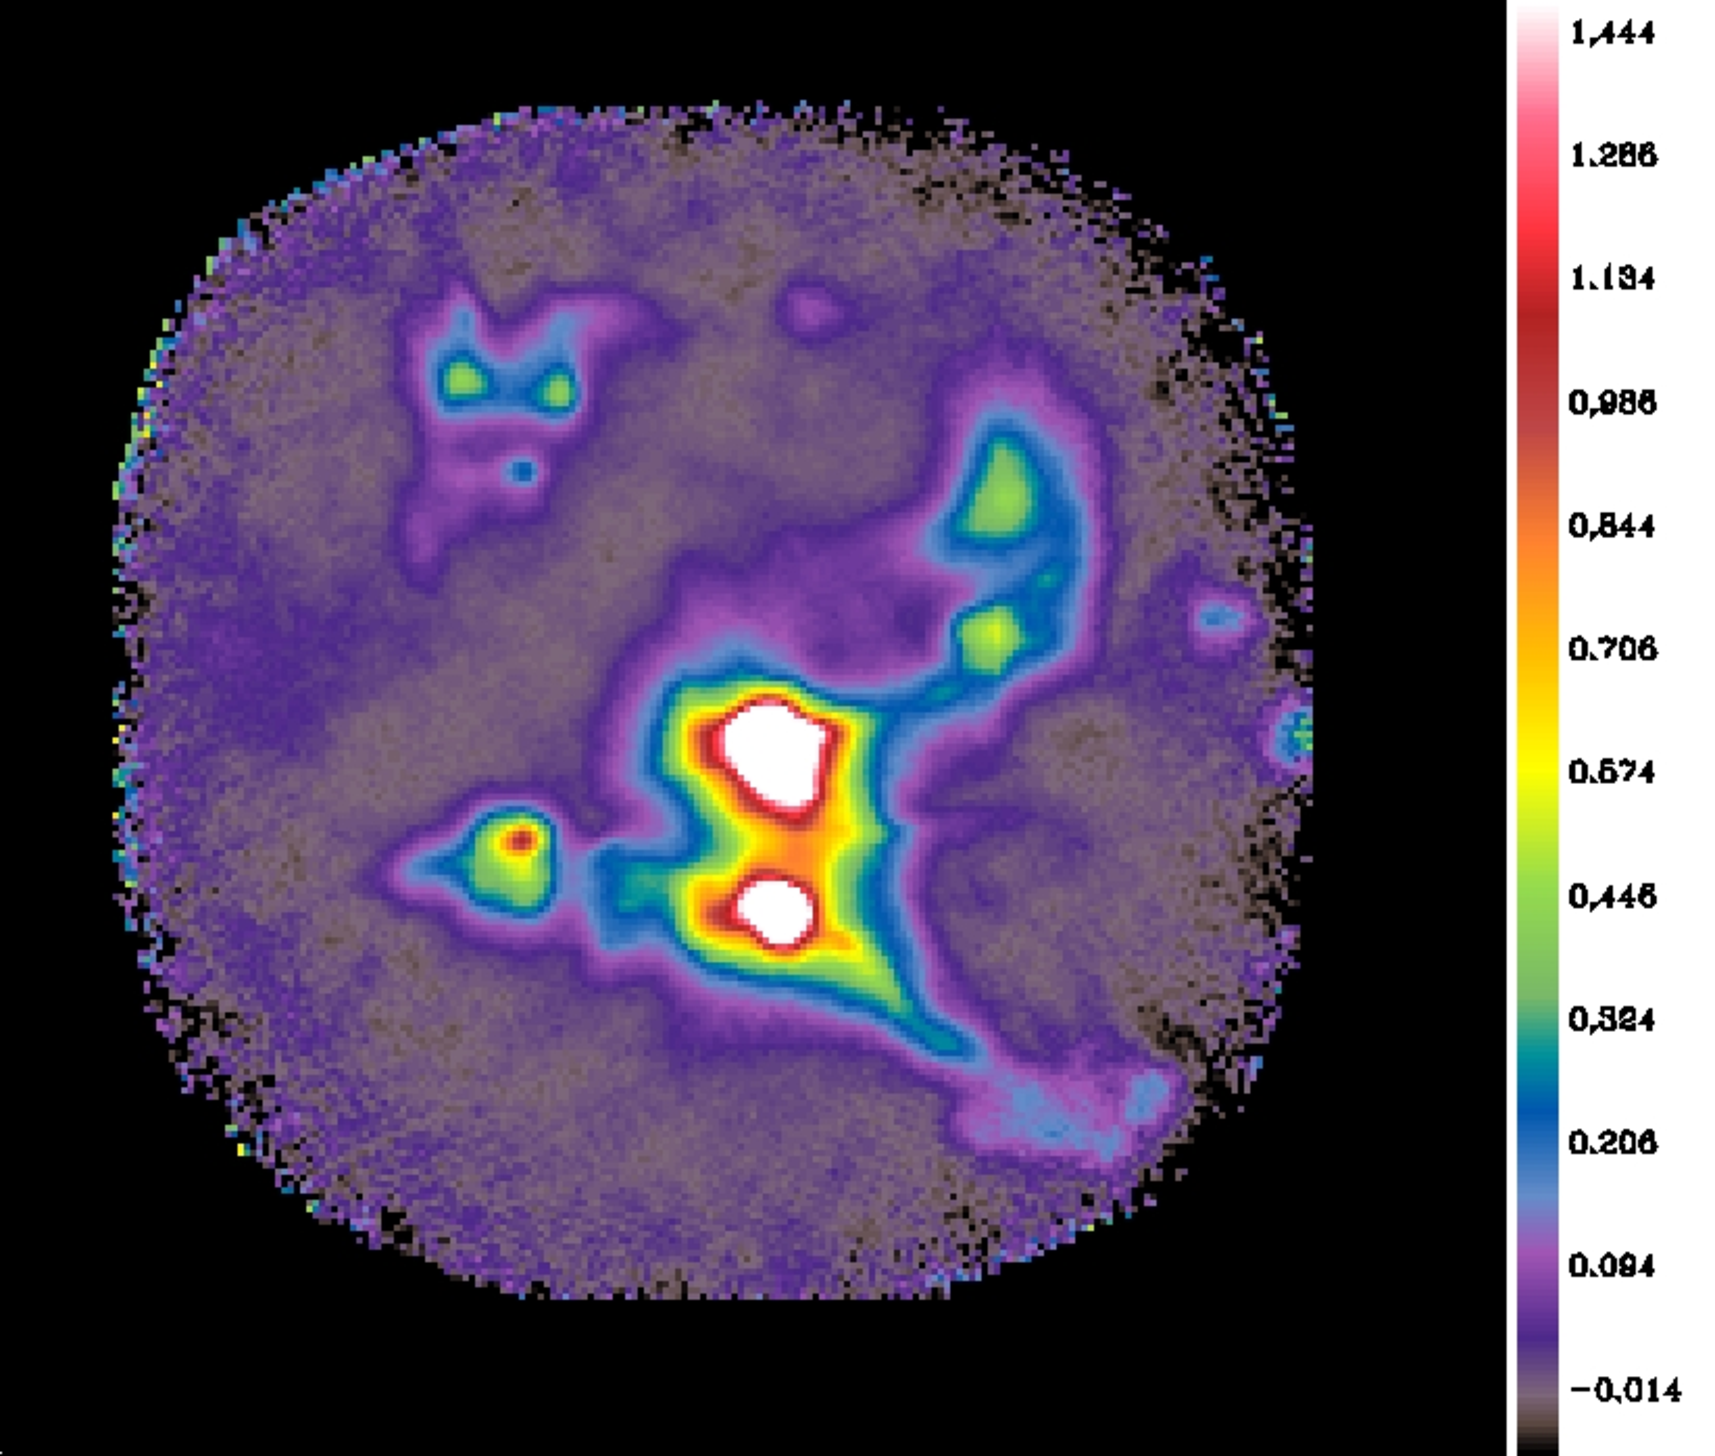
\includegraphics[width=0.48\textwidth,clip]{desert_fig3}%      
%  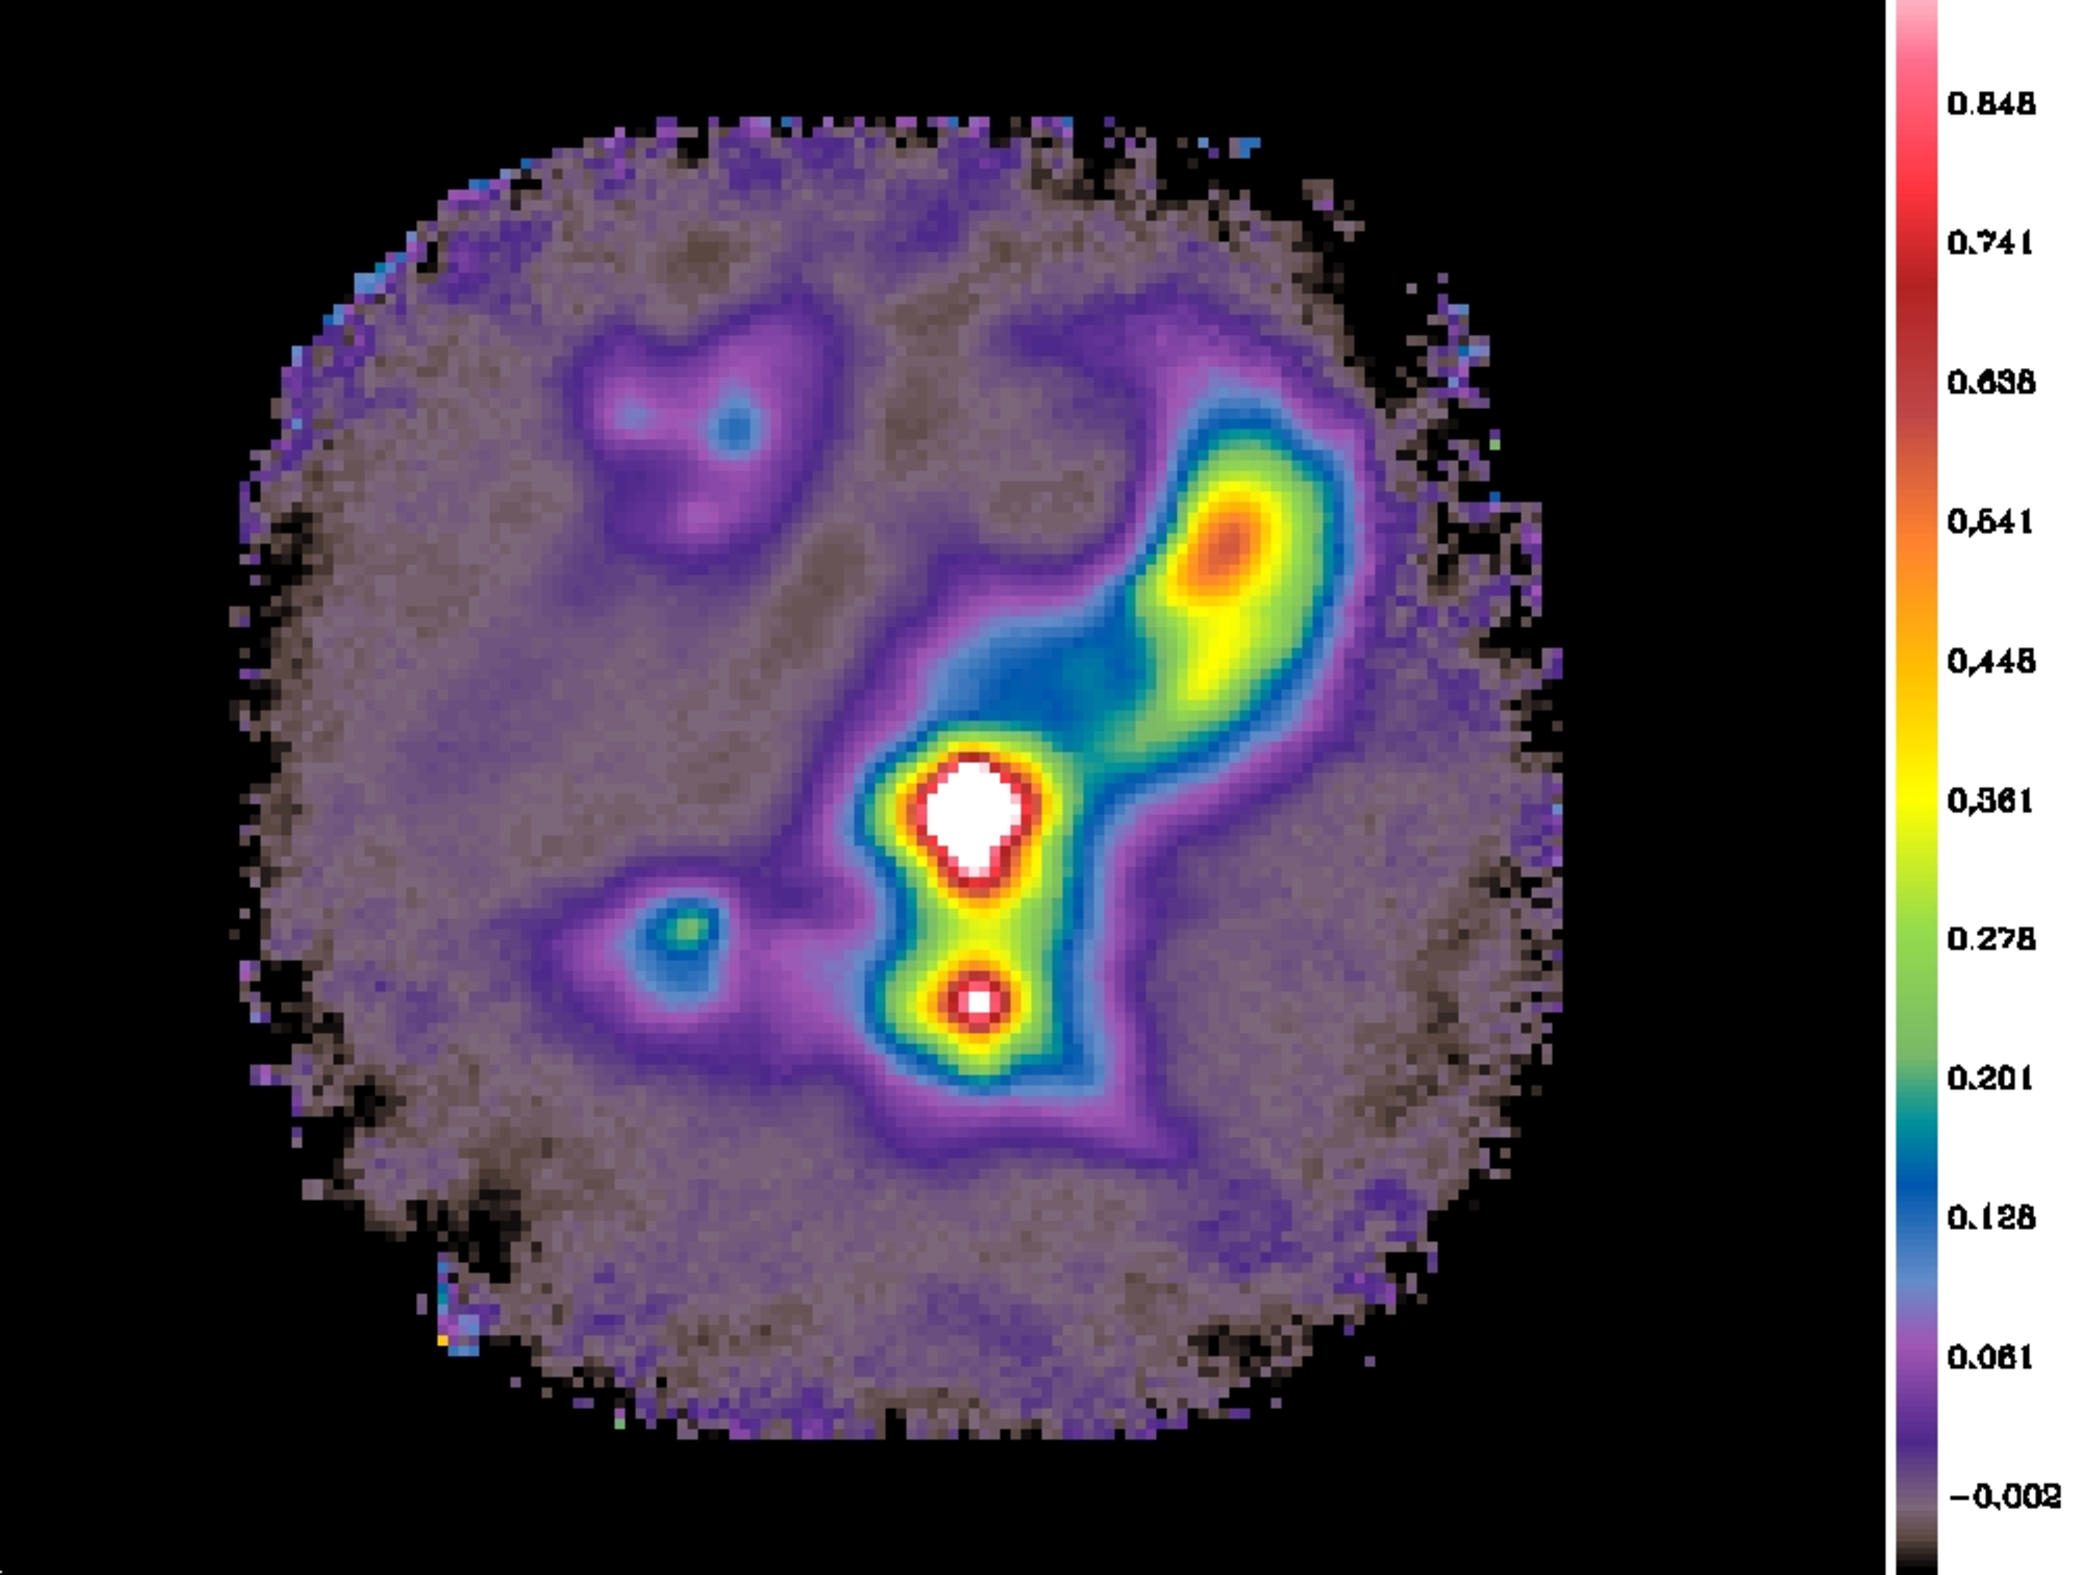
\includegraphics[width=0.48\textwidth,clip]{desert_fig4}      
% %% Note the ABSENCE of the extension .pdf  !
%  \caption{ RA-Dec maps centered on the ultracompact HII regions NGC~7538 at
%    {\bf Left:}~1.2~mm and {\bf Right:}~2~mm. The maps were obtained by using
%    the standard NIKA2 IDL-based pipeline and an adaptation of the Scanamorphos
%    map-making algorithm~\citep{2013PASP..125.1126R} to NIKA2. The integration
%    time was 12 minutes.  The size of the mapped square is 10~arcmin. The
%    brightness scale is linear and the maximum is at several Jy per beam. The
%    central calibrator is clearly surrounded by many other bright regions.}
%   \label{fig3-4}
% \end{figure}

\section{Conclusions}
% %%--------------------

% This is the conclusion of the article.
The NIKA2 commissionning is ongoing at the end of 2016. The final
configuration of the instrument, which includes improvements in optical
elements, filtering, readout electronics and the 2~mm array, still has to be
characterised. A science verification phase will begin in early 2017 and the
instrument could then be opened to the IRAM community. Five large programs of
guaranteed time will be pursued (along with open time proposals): 1) mapping
of the hot gas in fifty clusters of galaxies, as already performed on 6
clusters with the prototype
camera~\citep{adam2014,adam2015,adam2016,2016arXiv160707679R}, 2) a deep
survey down to the confusion limit, 3) mapping of nearby galaxies, 4) galactic
observations of star formation and dust properties, and 5) polarization of
star-forming regions. The observations with NIKA2 will provide several lists
of relevant targets to be explored by NOEMA.


% Optional acknowledgements
% -------------------------
\begin{acknowledgements}
  We would like to thank the IRAM staff for their support during the
  campaigns.  The NIKA dilution cryostat has been designed and built at the
  Institut N\'eel.  In particular, we acknowledge the crucial contribution of
  the Cryogenics Group, and in particular Gregory Garde, Henri Rodenas, Jean
  Paul Leggeri, Philippe Camus.  This work has been partially funded by the
  Foundation Nanoscience Grenoble, the LabEx FOCUS ANR-11-LABX-0013 and the
  ANR under the contracts "MKIDS", "NIKA" and ANR-15-CE31-0017.  This work has
  benefited from the support of the European Research Council Advanced Grant
  ORISTARS under the European Union's Seventh Framework Programme (Grant
  Agreement no. 291294).  We acknowledge fundings from the ENIGMASS French
  LabEx (R. A. and F. R.), the CNES post-doctoral fellowship program (R. A.),
  the CNES doctoral fellowship program (A. R.) and the FOCUS French LabEx
  doctoral fellowship program (A. R.).
\end{acknowledgements}

%%-----------------------------
%%   Bibliography
%%-----------------------------
%%
%% The reference list should contain all the references cited in the text, ordered alphabetically by surname (with
%% initials following). If there are several references to the same first author, they should be entered according
%% to the following scheme:
%% 1. One author: chronologically
%% 2. Author, one co-author: alphabetically by co-author, then chronologically
%% 3. Author, two or more co-authors: chronologically.
%%
%% Please note that for papers that have more than five authors, only the first three should be given, followed
%% by "et al."
%%
%% The format for references is the one adopted by A&A (see the example below).
%%
%% To set the reference list in the proper A&A format, we encourage you to use BibTEX and the natbib
%% package instead of the standard 'thebibliography' environment.
%%

%\begin{thebibliography}{}
%\bibitem[Bohr et al.(1992)]{Bohr26} Bohr, N., Einstein, A., \& Fermi, E. 1992, MNRAS, 301, 257
%\bibitem[Curie \& Curie(1991)]{Curie91} Curie, M., \& Curie, P. 1991, A\&A, 248, 612
%\bibitem[de Gaulle(1996)]{de Gaulle96} de Gaulle, C. 1996, Solar Phys. (Oxford Univ. Press, Oxford)
%\bibitem[Einstein(1926)]{Einstein26} Einstein, A. 1926, ApJ, 63, 196 (Paper~II) 
%\bibitem[Einstein \& Strauss(1945)]{1945RvMP...17..120E} Einstein, A., 
%\& Strauss, E.G. 1945, Rev. Mod. Phys., 17, 120
%\bibitem[Kafka et al.(1924)]{Kafka24} Kafka, F., Laurel, S., Hardy, O. et al. 1924, A\&A, 248, 612
%\bibitem[Laurel \& Hardy(1994)]{Laurel94} Laurel, S., \& Hardy, O. 1994, Active Driking, in The Evolution
% and Distribution of Beverages, eds. W. Churchill, F. D. Roosevelt, \& A. Capone (Chicago: Bourbon Distilleries Inc.), p. 234 
%\end{thebibliography}

%% The following lines are required when using BibTEX (strongly encouraged!):
\bibliographystyle{aa}  % A&A bibliography style file (aa.bst)
\bibliography{desert} % your references in file: Yourfile.bib


%
\end{document}
%%%%%%%%%%%%%%%%%%%%%%%%%%%%%%%%%%%%%%%%%%%%%%%%%%%%%%%%%%%%%%%%%%
